\chapter{Bus Stop Detection}
\label{cha:bus-stop-detection}

The first high-level problem is the problem with inaccurate bus stop detections.
This causes the system to occasionally miss bus stops, which results in faulty or incomplete journeys.
Incomplete journeys require more pre-processing to be done in order to use the data.
Another problem with the existing bus stop detection algorithm is that bus stop coordinates are pre-determined, meaning that they do not always represent the actual bus stop.
This introduces an overhead to the system, where bus stop coordinates need to be updated in order to continue to provide accurate detection of bus stops.

\begin{figure}[ht!]
    \centering
    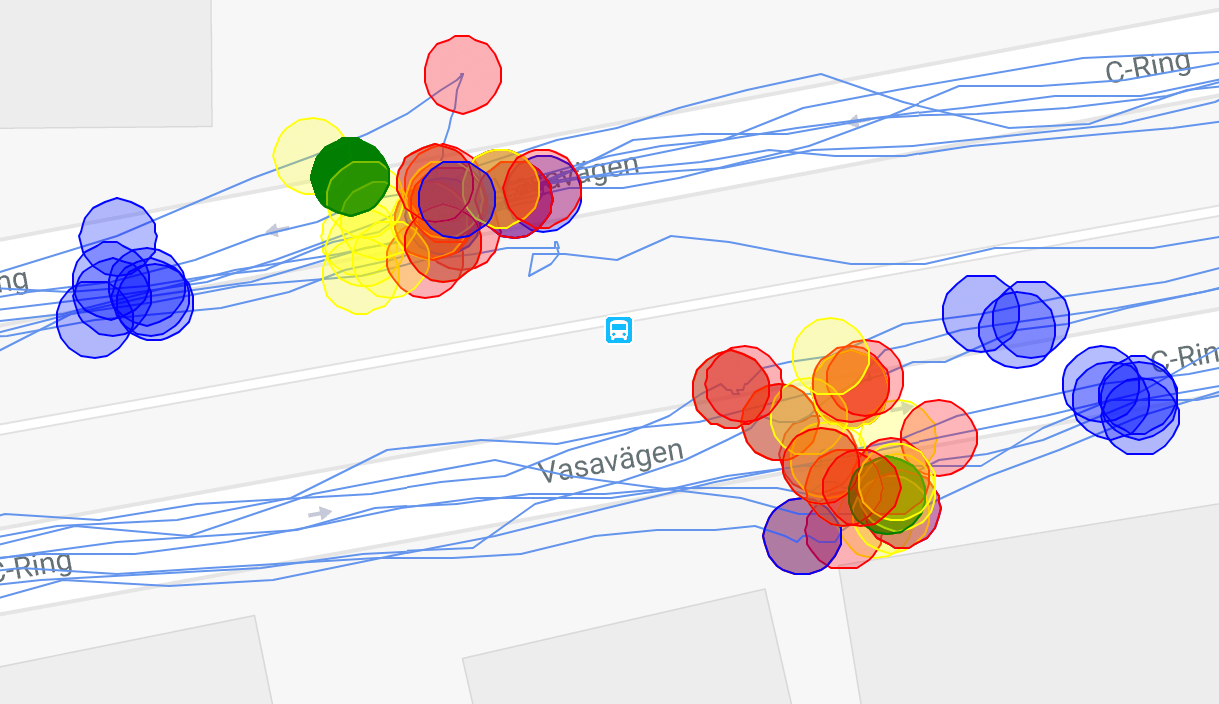
\includegraphics[width=0.9\textwidth]{figures/bus_stops}
    \caption{Output from the Bus Stop Detection Algorithm from the "Internal Analysis" component.
    The green circle are the pre-determined coordinates for the bus stop.
    The bus stop shown has two modes, depending on if the bus travels west (top road) or east (bottom road).
    The red and yellow clusters are the GPS positions of the bus when it arrives to the bus stop.
    The blue clusters are the GPS positions of the buses departing from the bus stop.
    }
    \label{fig:bus-stop-clusters}
\end{figure}

Figure \ref{fig:bus-stop-clusters} shows the results from the existing Bus Stop Detection Algorithm of the "Internal Analysis" component.
Each bus produces seven GPS coordinates for each bus stop: one blue, two red, two yellow, and one green.
The green GPS coordinate is always the same between all buses for each bus stop; it is the pre-determined coordinate for the bus stop.
The blue GPS coordinate is the position of the bus when it departures from the bus stop (the last positional update within a pre-determined radius of the bus stop).
The red and yellow coordinates are the positions of the buses when the system determines that they have arrived (stopped) at the bus stop.
Due to lacking documentation, the difference between the red and yellow coordinates are unclear as they are occasionally identical, but not always (as shown in the figure).
The existing bus stop detection algorithm thus checks within a pre-determined radius around the green GPS coordinate for updates from buses.
When the first positional update from the bus is received, the system tracks the bus and waits for it to stop.
Upon stopping, the bus is determined to have arrived at the bus stop.
When the bus starts again, the system continues to track it and reports when the bus has left the radius of the bus stop.
The blue GPS coordinate shows where this happens. 